\begin{frame}{Feature Distribution Smoothing (FDS)}
	\begin{itemize}\setlength\itemsep{1.5em}
		\item<2-> Starting points
		\begin{enumerate}
			\item<2-> Continuity in the \textbf{target} space $\longleftrightarrow$ Continuity in the \textbf{feature} space
			\item<3-> Data balance $\Longrightarrow$ close feature statistics of nearby targets
		\end{enumerate}
		\item<4-> Feature statistics: mean and variance w.r.t. each bin
		\begin{equation*}
			\{\bm{\mu}_b,\bm{\sigma}_b\}_{b=1}^B
		\end{equation*}
		\item<5-> (next slides) Feature statistics similarity: cosine similarity of \\feature statistics between one anchor bin $b_0$ and all other bins
		\begin{itemize}
			\item $b_0 = 0, 30, 60, 90$ (age): chosen anchor bins
			\item different target densities: \\many ($>$100), medium (20-100), few~($<$20) examples
			\item task: person's picture $\longrightarrow$ person's age
			\item data source: IMDB-WIKI
		\end{itemize}
	\end{itemize}
\end{frame}

\begin{frame}{Feature statistics similarity (1/4)}{Anchor age 30}
	\begin{figure}[h]
		\begin{subfigure}{0.48\textwidth}
			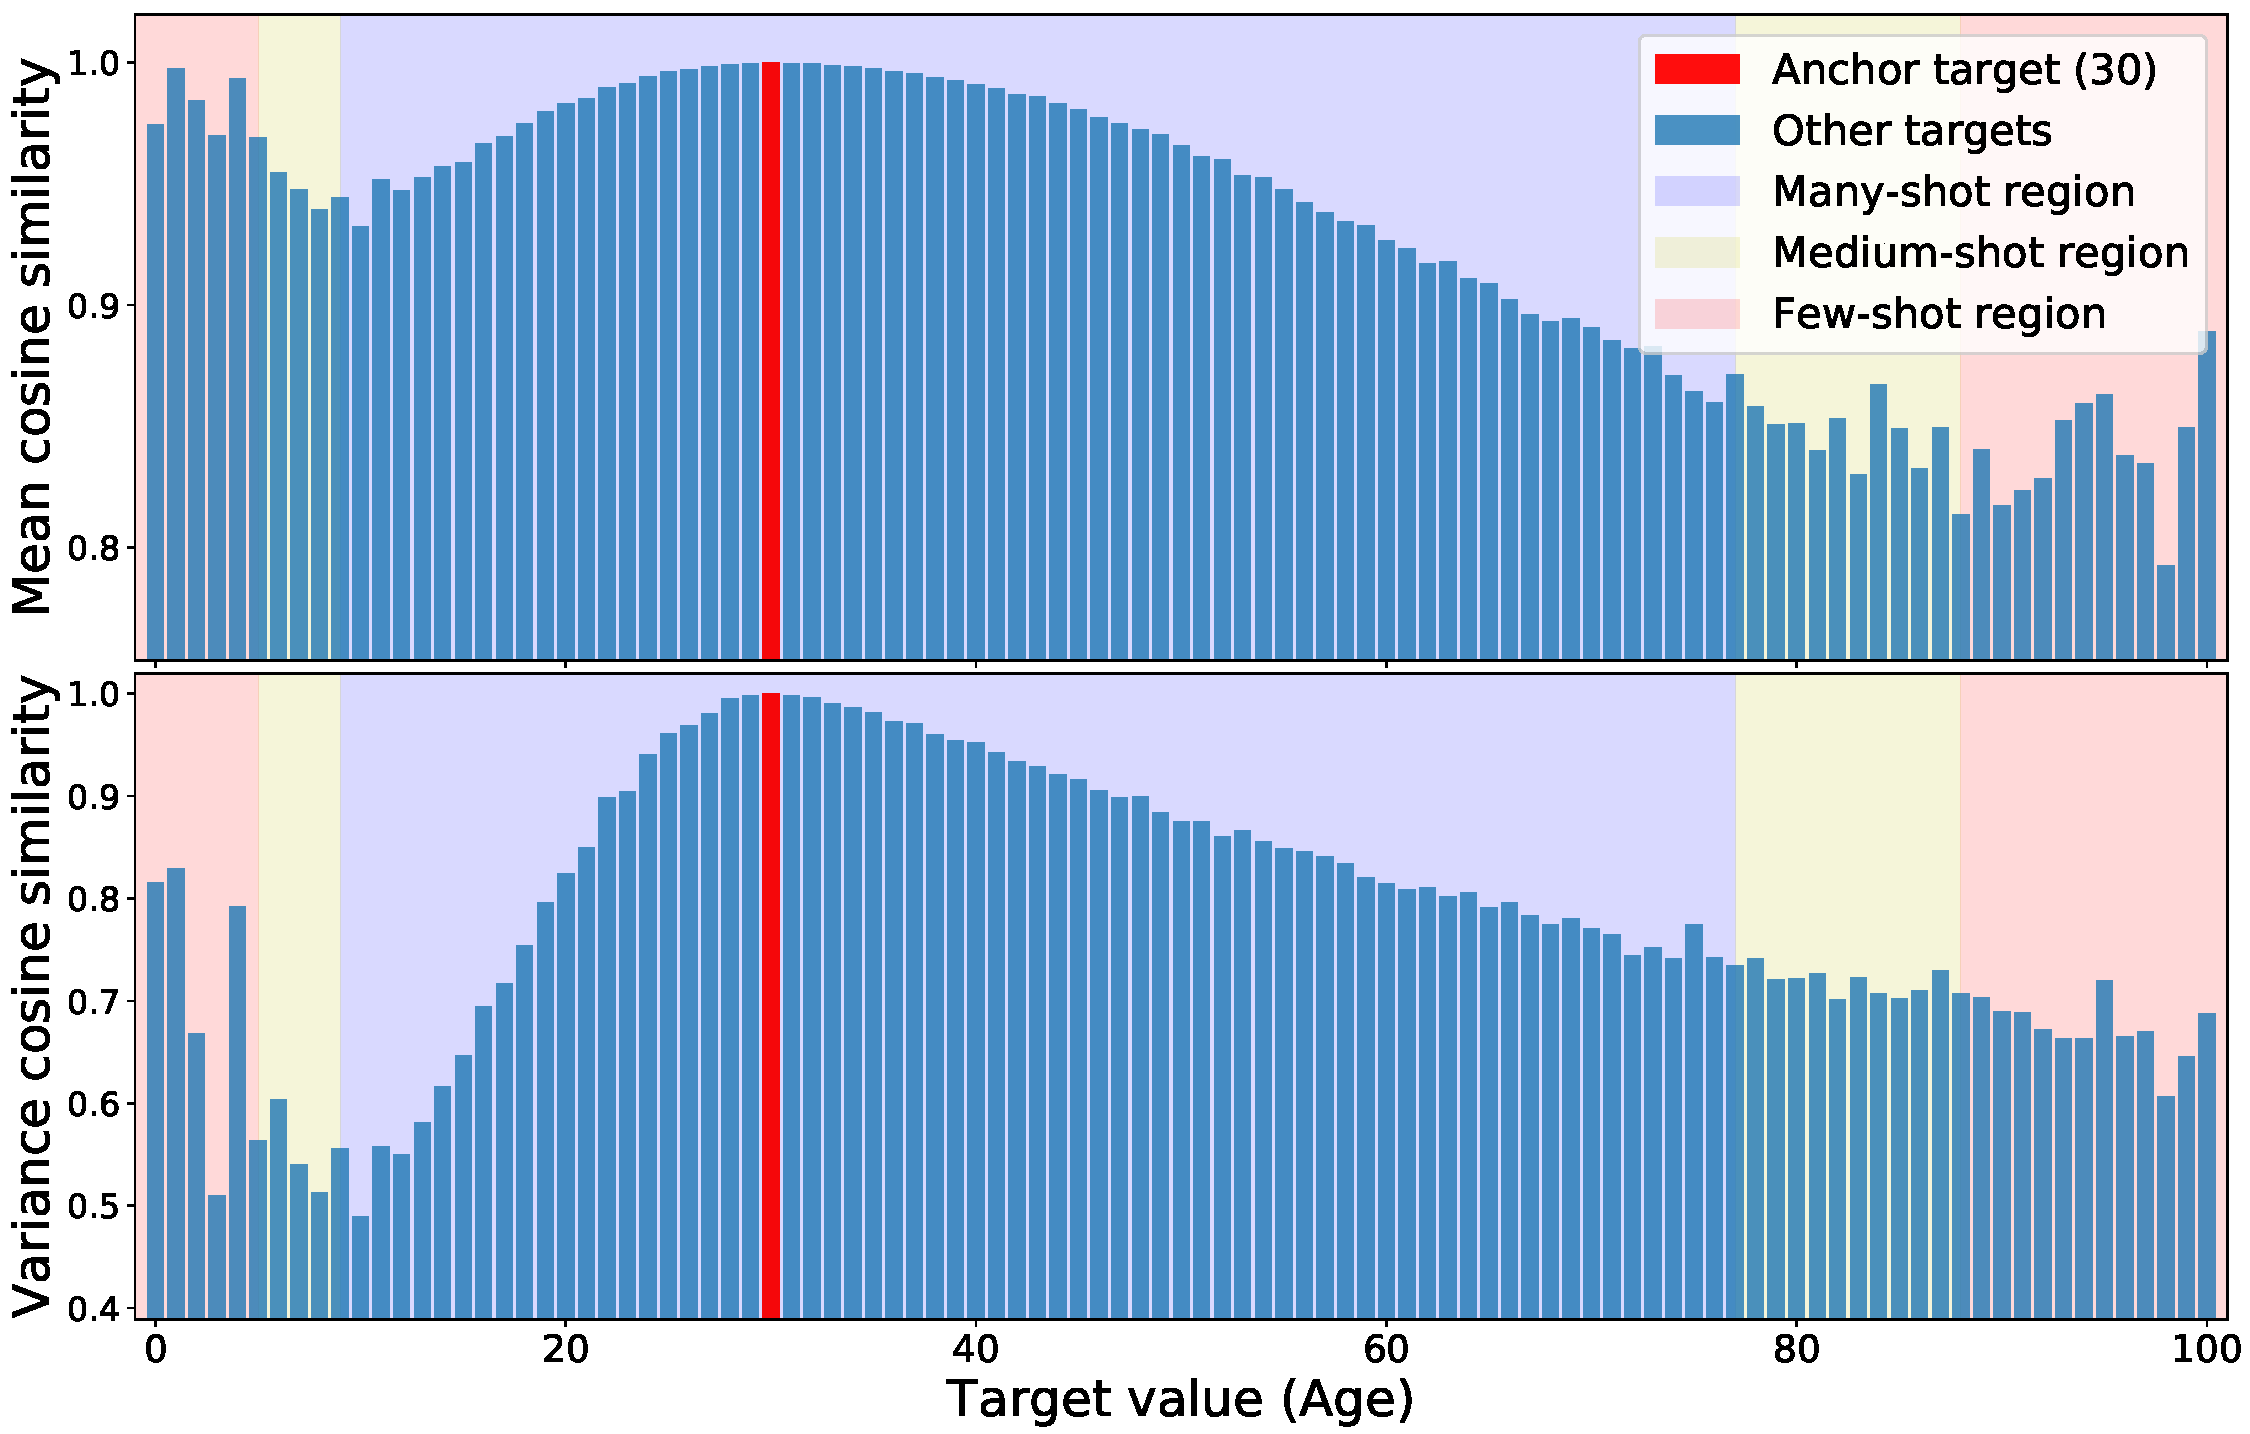
\includegraphics[width=\linewidth]{images/feat_sim_fds_base_30.pdf}
			\caption{Baseline}
		\end{subfigure}\hspace{1em}%
		\begin{subfigure}{0.48\textwidth}
			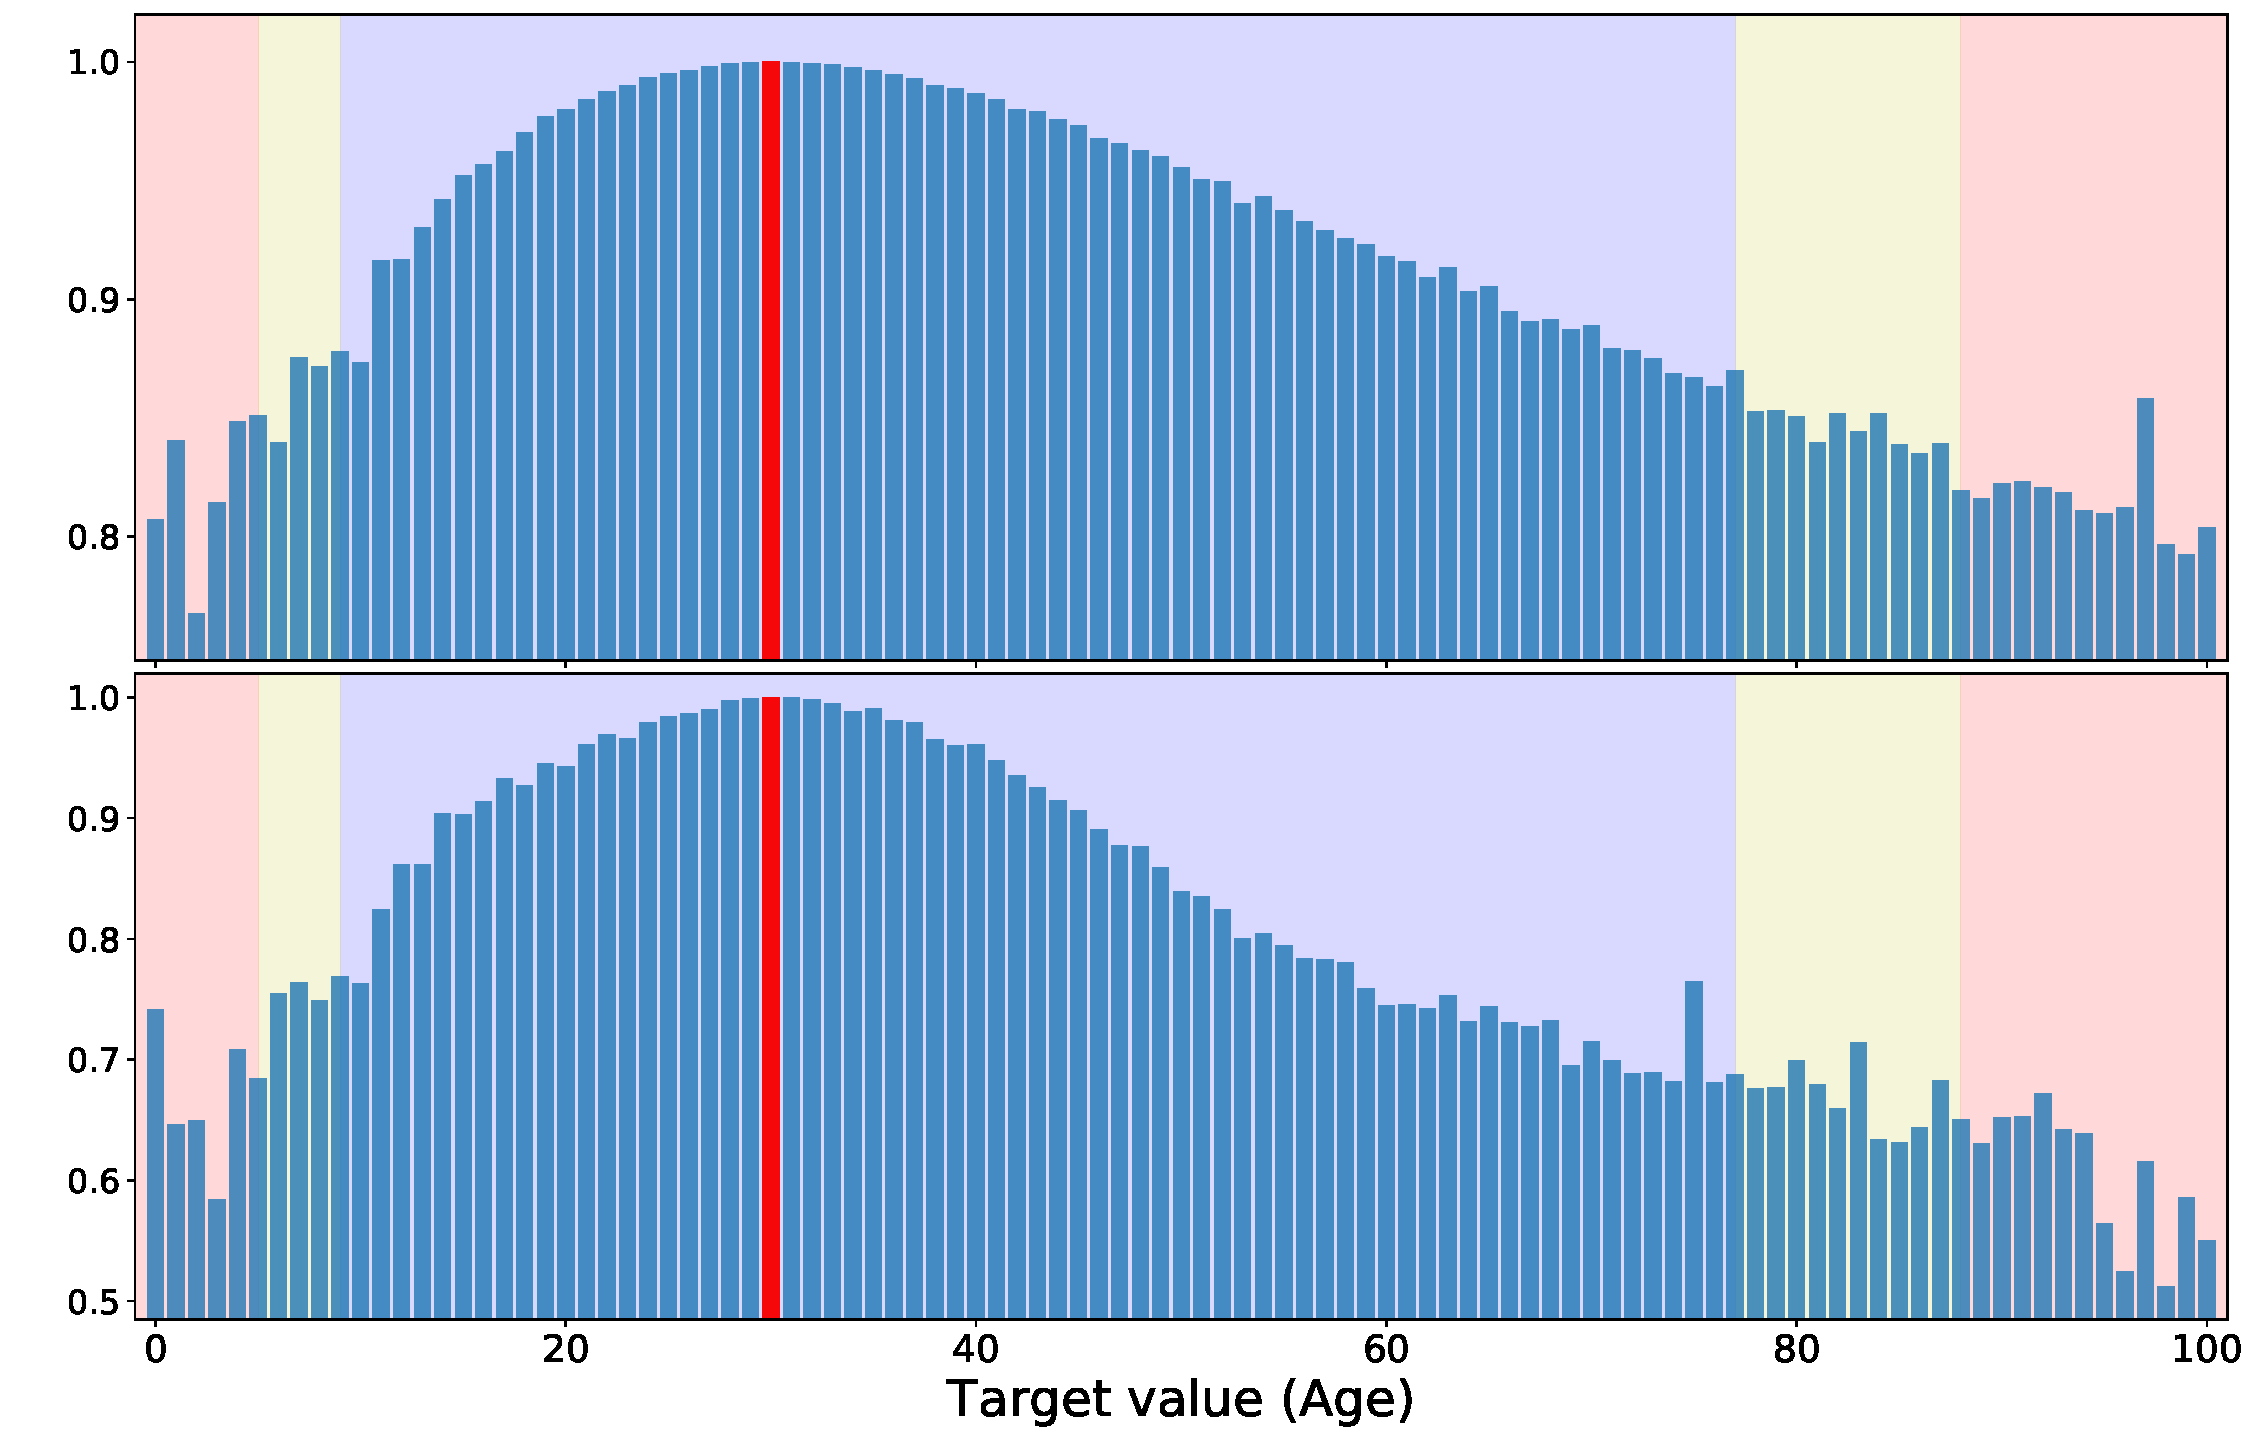
\includegraphics[width=\linewidth]{images/feat_sim_fds_ours_30.pdf}
			\caption{FDS}
		\end{subfigure}
		%\caption{}
	\end{figure}
	\vspace{-1em}
	\begin{columns}
		\footnotesize
		\begin{column}{0.5\textwidth}
			\begin{itemize}
				\item High similarity in neighbourhood
				\item \red{High similarities with further regions}
				\item \red{Lower similarities with some closer regions}
			\end{itemize}
		\end{column}
		\begin{column}{0.5\textwidth}
			\begin{itemize}
				\item Improved feature statistics calibration:
				\begin{itemize}
					\vspace{-1.5em}
					\scriptsize
					\item High similarity only in neighbourhood
					\item ``The further the region the lower the similarity''
					\item More gradual similarity change
				\end{itemize}
			\end{itemize}
		\end{column}
	\end{columns}
	\credit{Image}{yang2021delving}
\end{frame}

\begin{frame}{Feature statistics similarity (2/4)}{Anchor age 60}
	\begin{figure}[h]
		\begin{subfigure}{0.48\textwidth}
			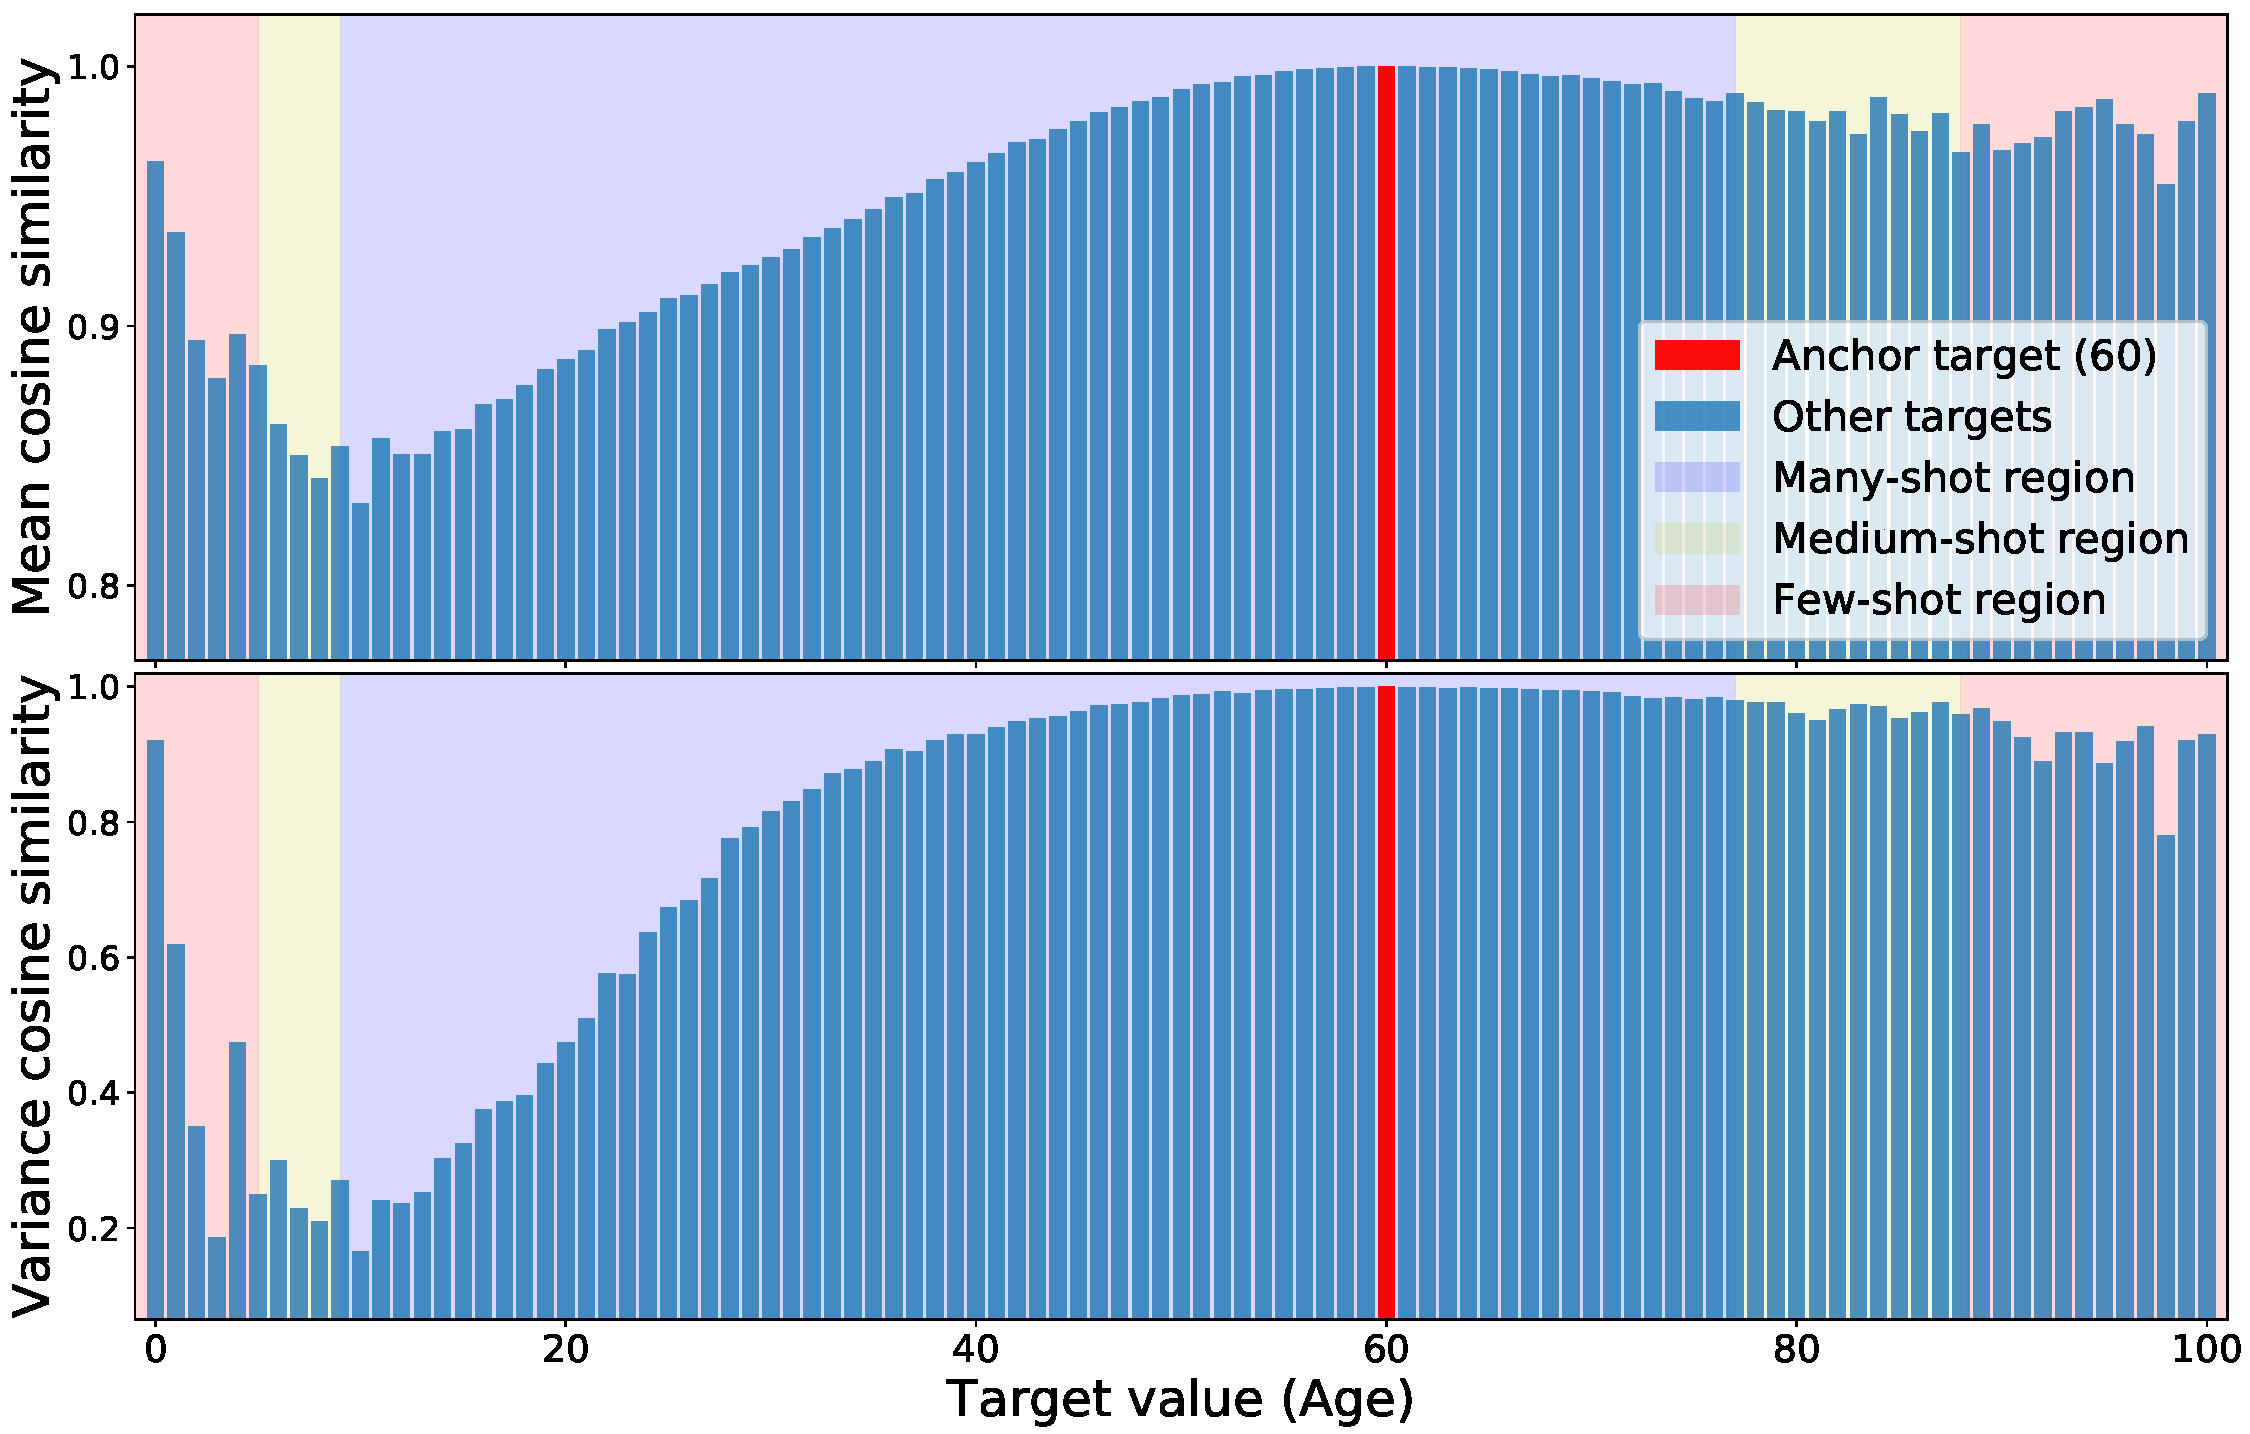
\includegraphics[width=\linewidth]{images/feat_sim_fds_base_60.pdf}
			\caption{Baseline}
		\end{subfigure}\hspace{1em}%
		\begin{subfigure}{0.48\textwidth}
			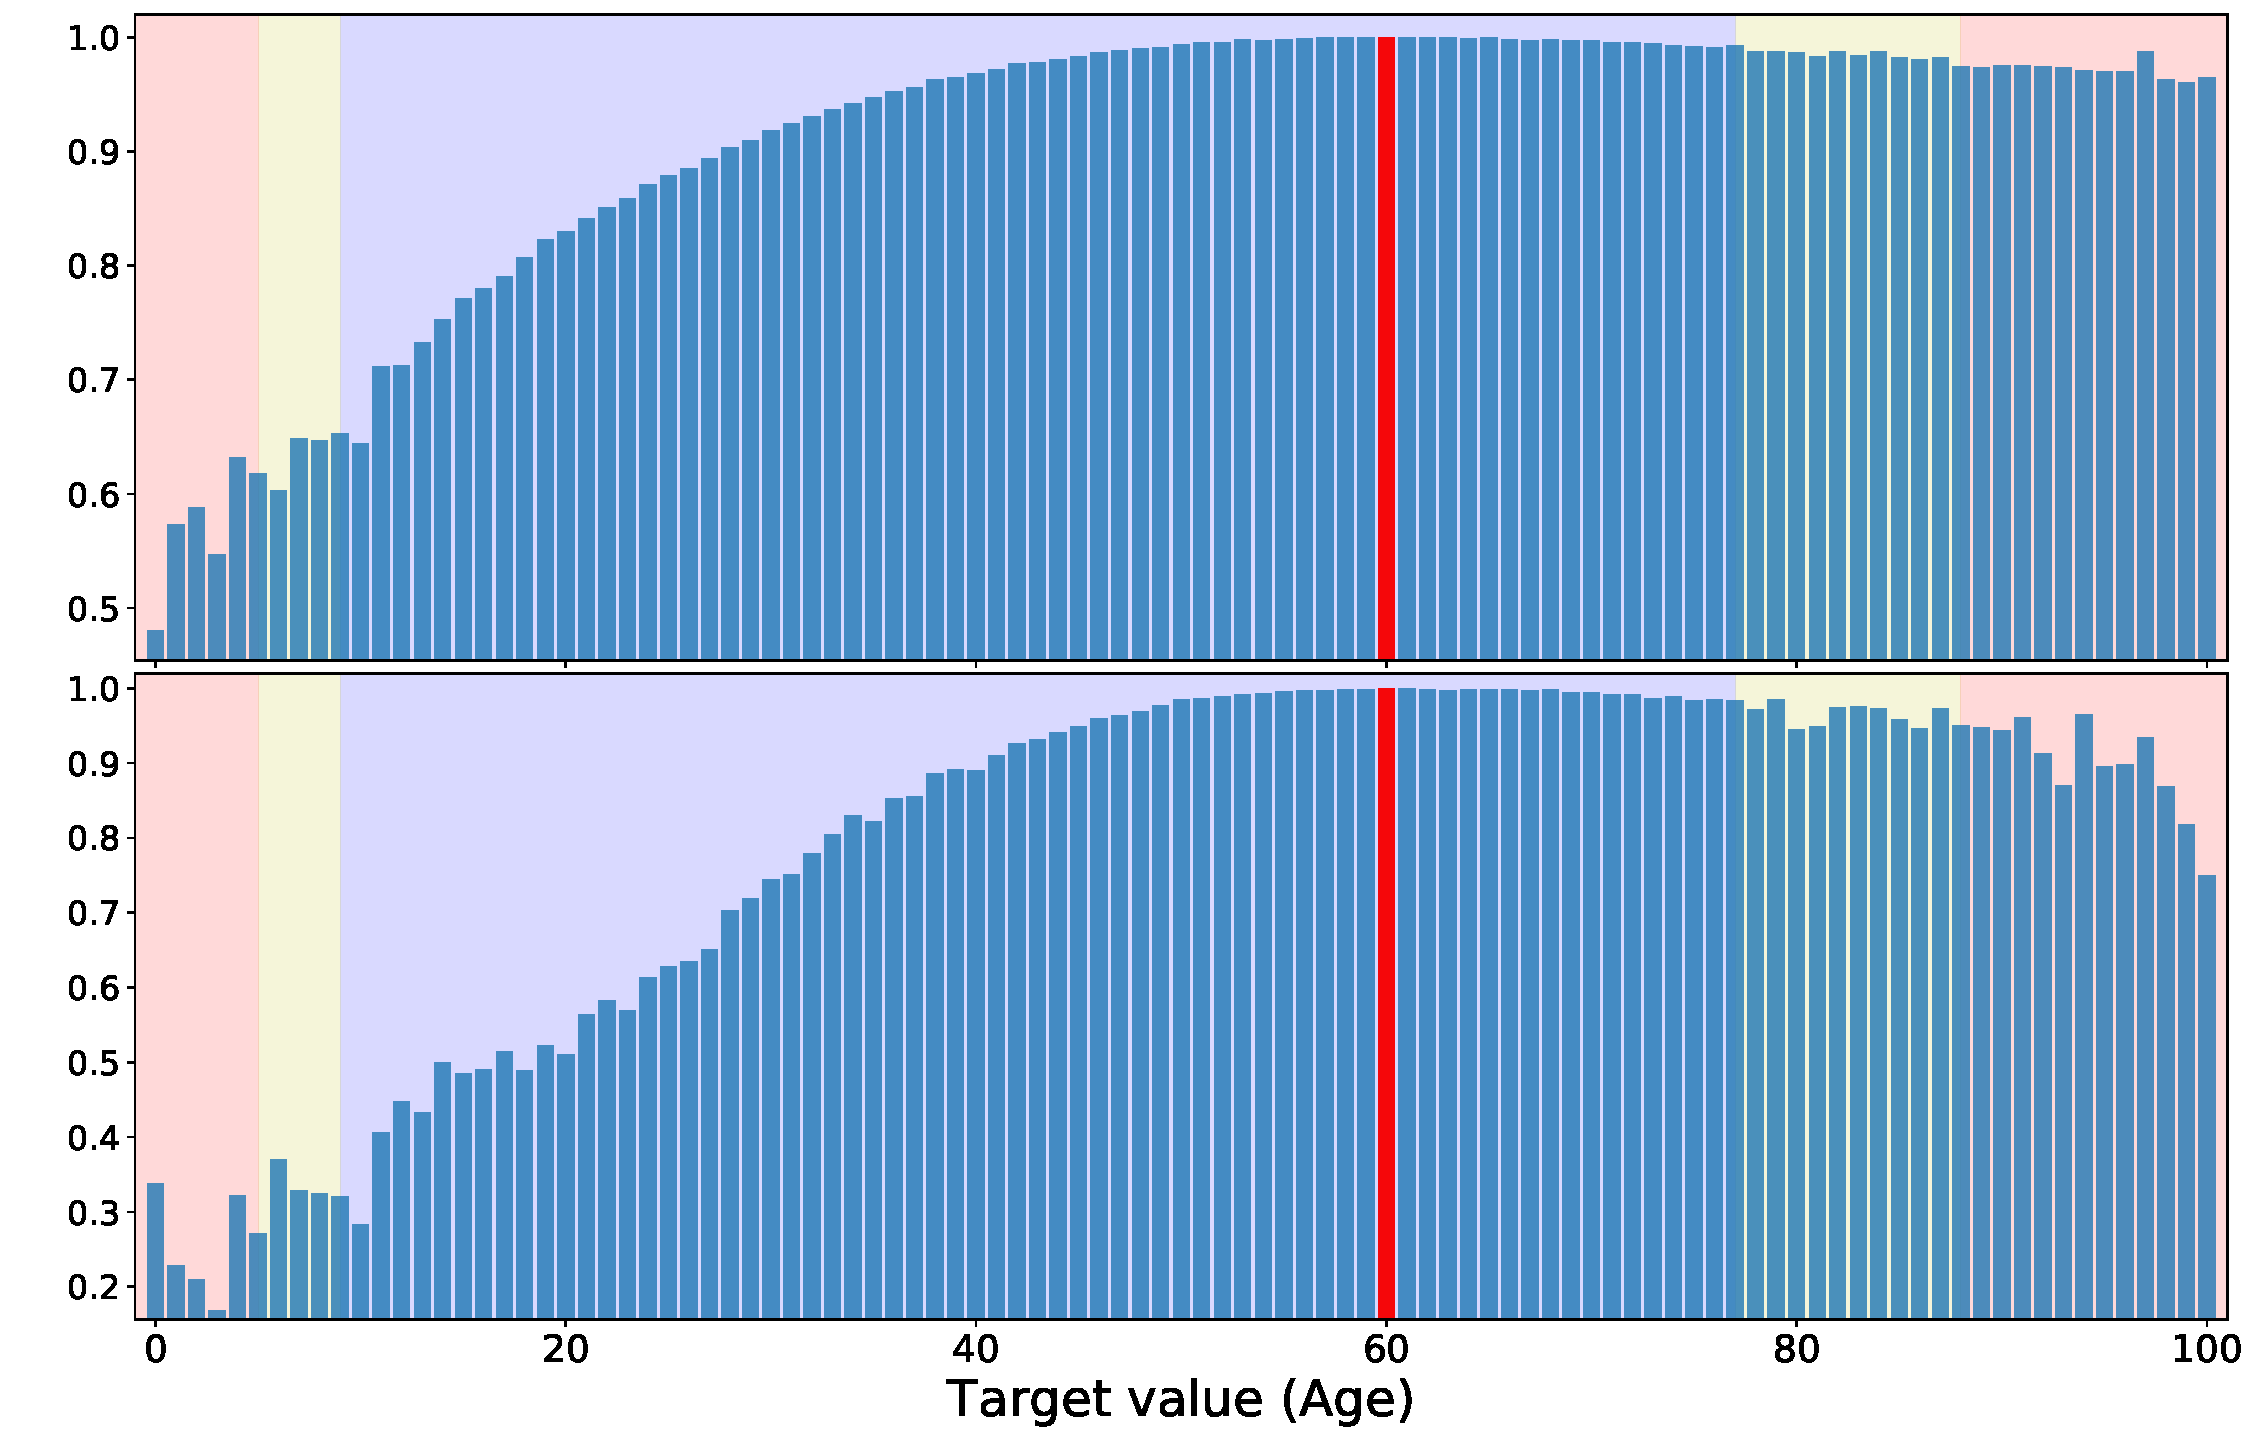
\includegraphics[width=\linewidth]{images/feat_sim_fds_ours_60.pdf}
			\caption{FDS}
		\end{subfigure}
		%\caption{}
	\end{figure}
	\vspace{-1em}
	\begin{columns}
		\footnotesize
		\begin{column}{0.5\textwidth}
			\begin{itemize}
				\item High similarity in neighbourhood
				\item \red{High similarities with further regions}
				\item \red{Lower similarities with some closer regions}
			\end{itemize}
		\end{column}
		\begin{column}{0.5\textwidth}
			\begin{itemize}
				\item Improved feature statistics calibration:
				\begin{itemize}
					\vspace{-1.5em}
					\scriptsize
					\item High similarity only in neighbourhood
					\item ``The further the region the lower the similarity''
					\item More gradual similarity change
				\end{itemize}
			\end{itemize}
		\end{column}
	\end{columns}
	\credit{Image}{yang2021delving}
\end{frame}

\begin{frame}{Feature statistics similarity (3/4)}{Anchor age 0}
	\begin{figure}[h]
		\begin{subfigure}{0.48\textwidth}
			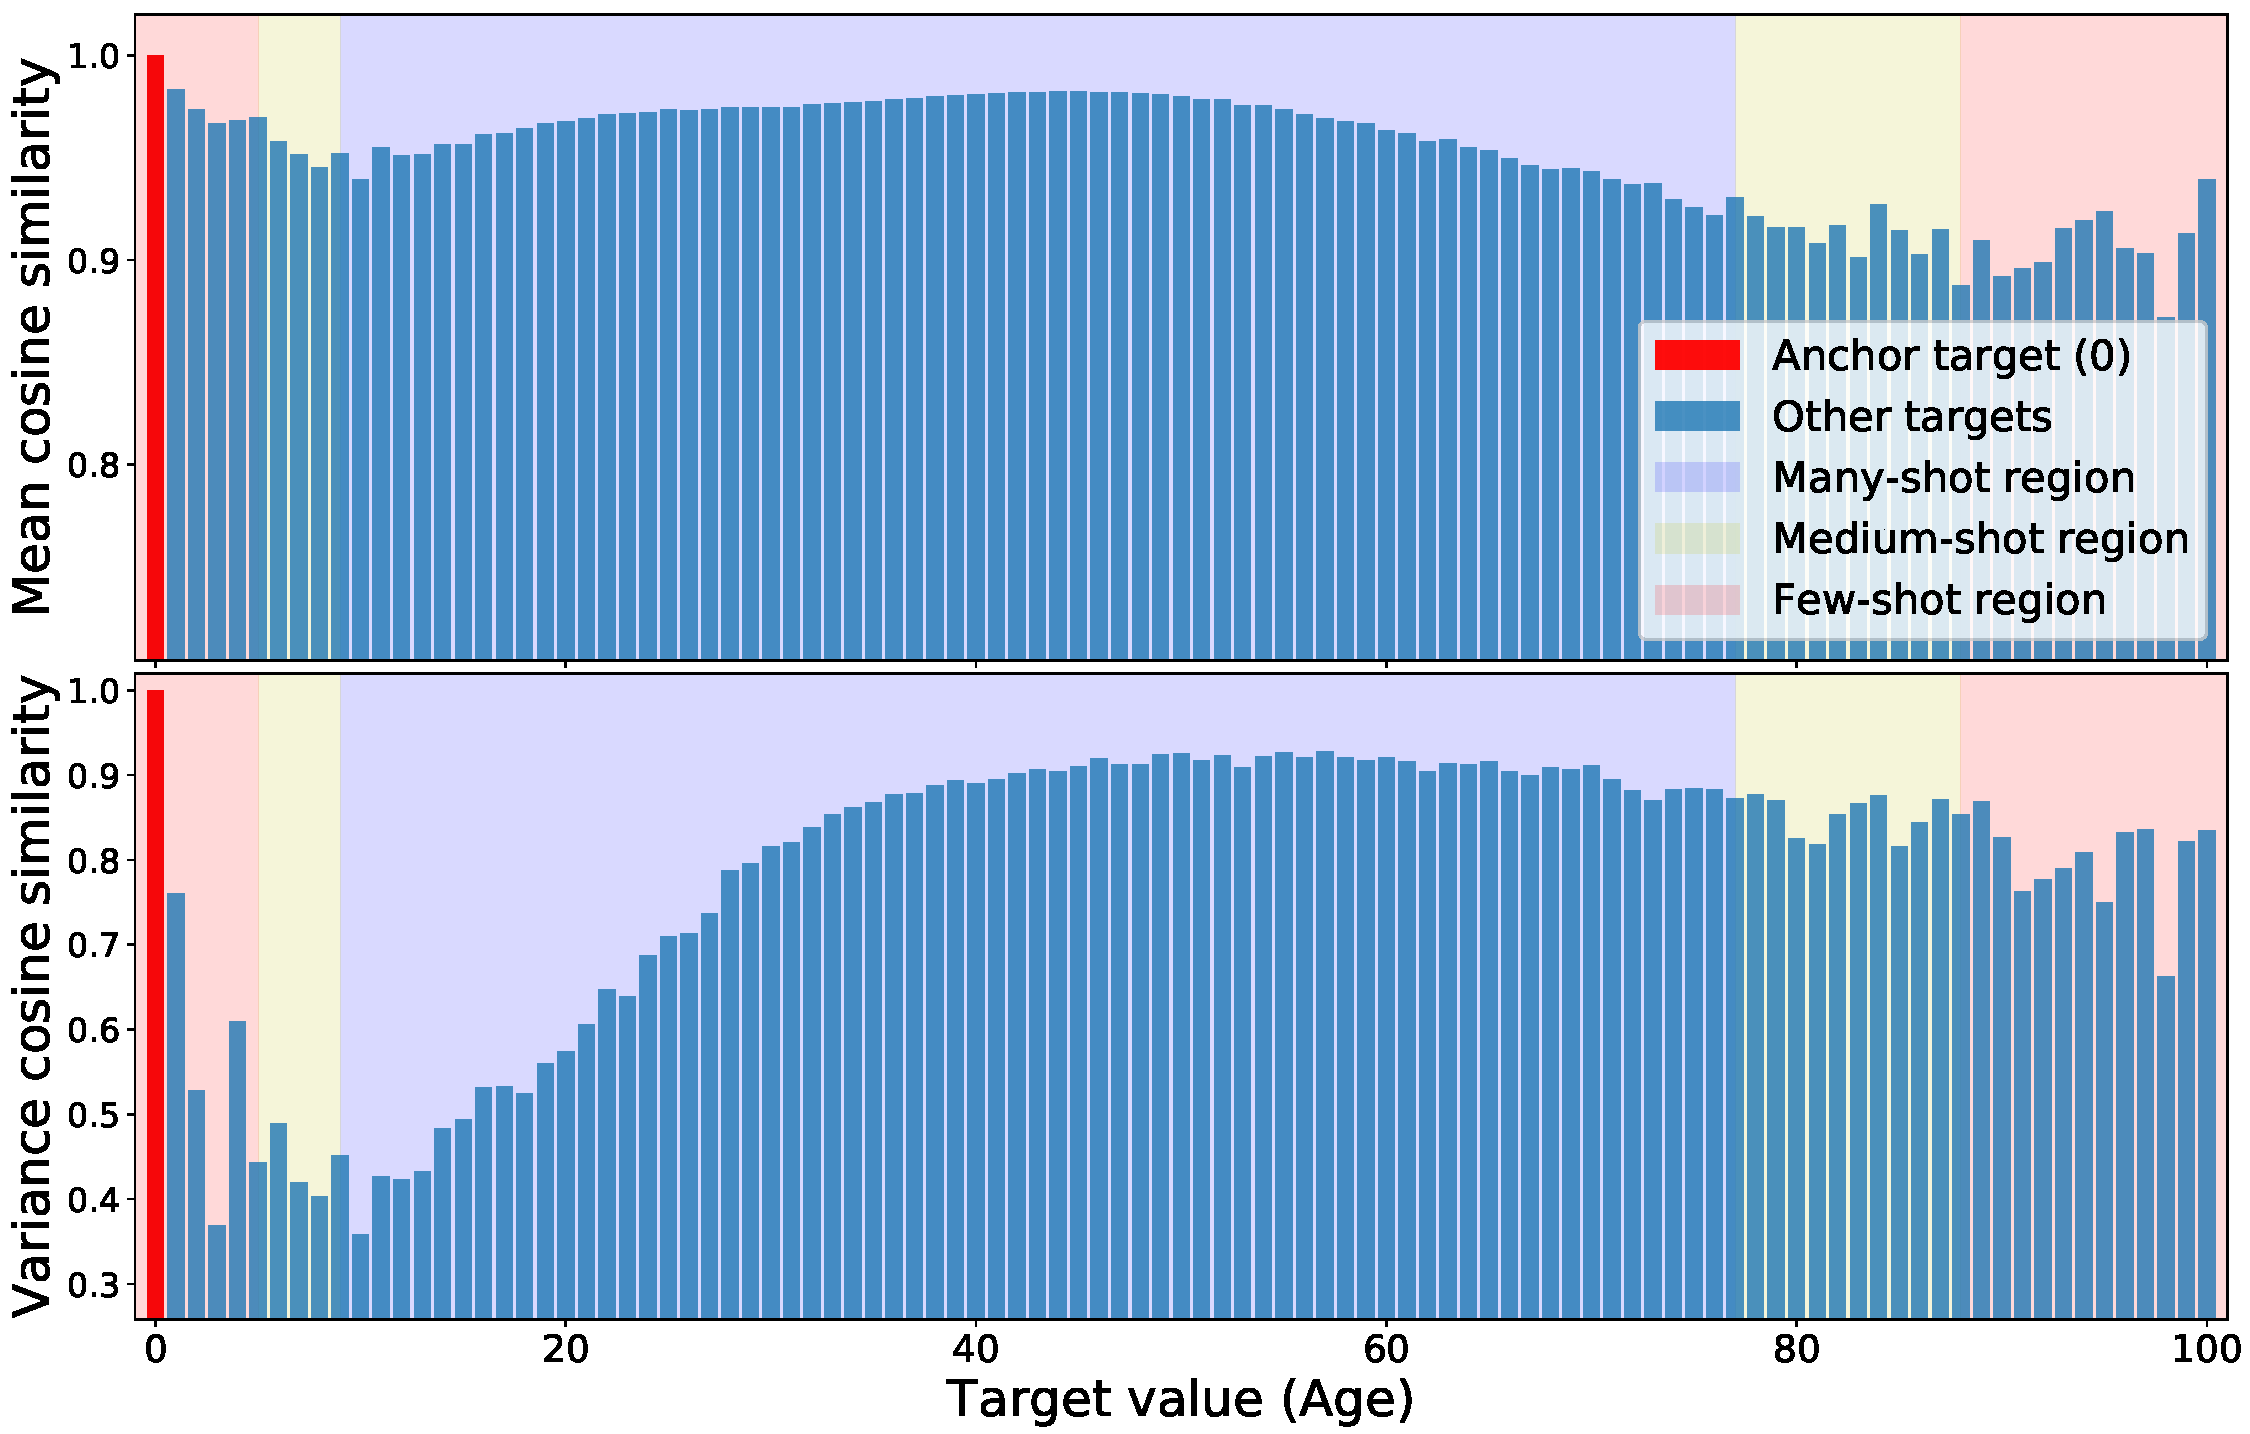
\includegraphics[width=\linewidth]{images/feat_sim_fds_base_0.pdf}
			\caption{Baseline}
		\end{subfigure}\hspace{1em}%
		\begin{subfigure}{0.48\textwidth}
			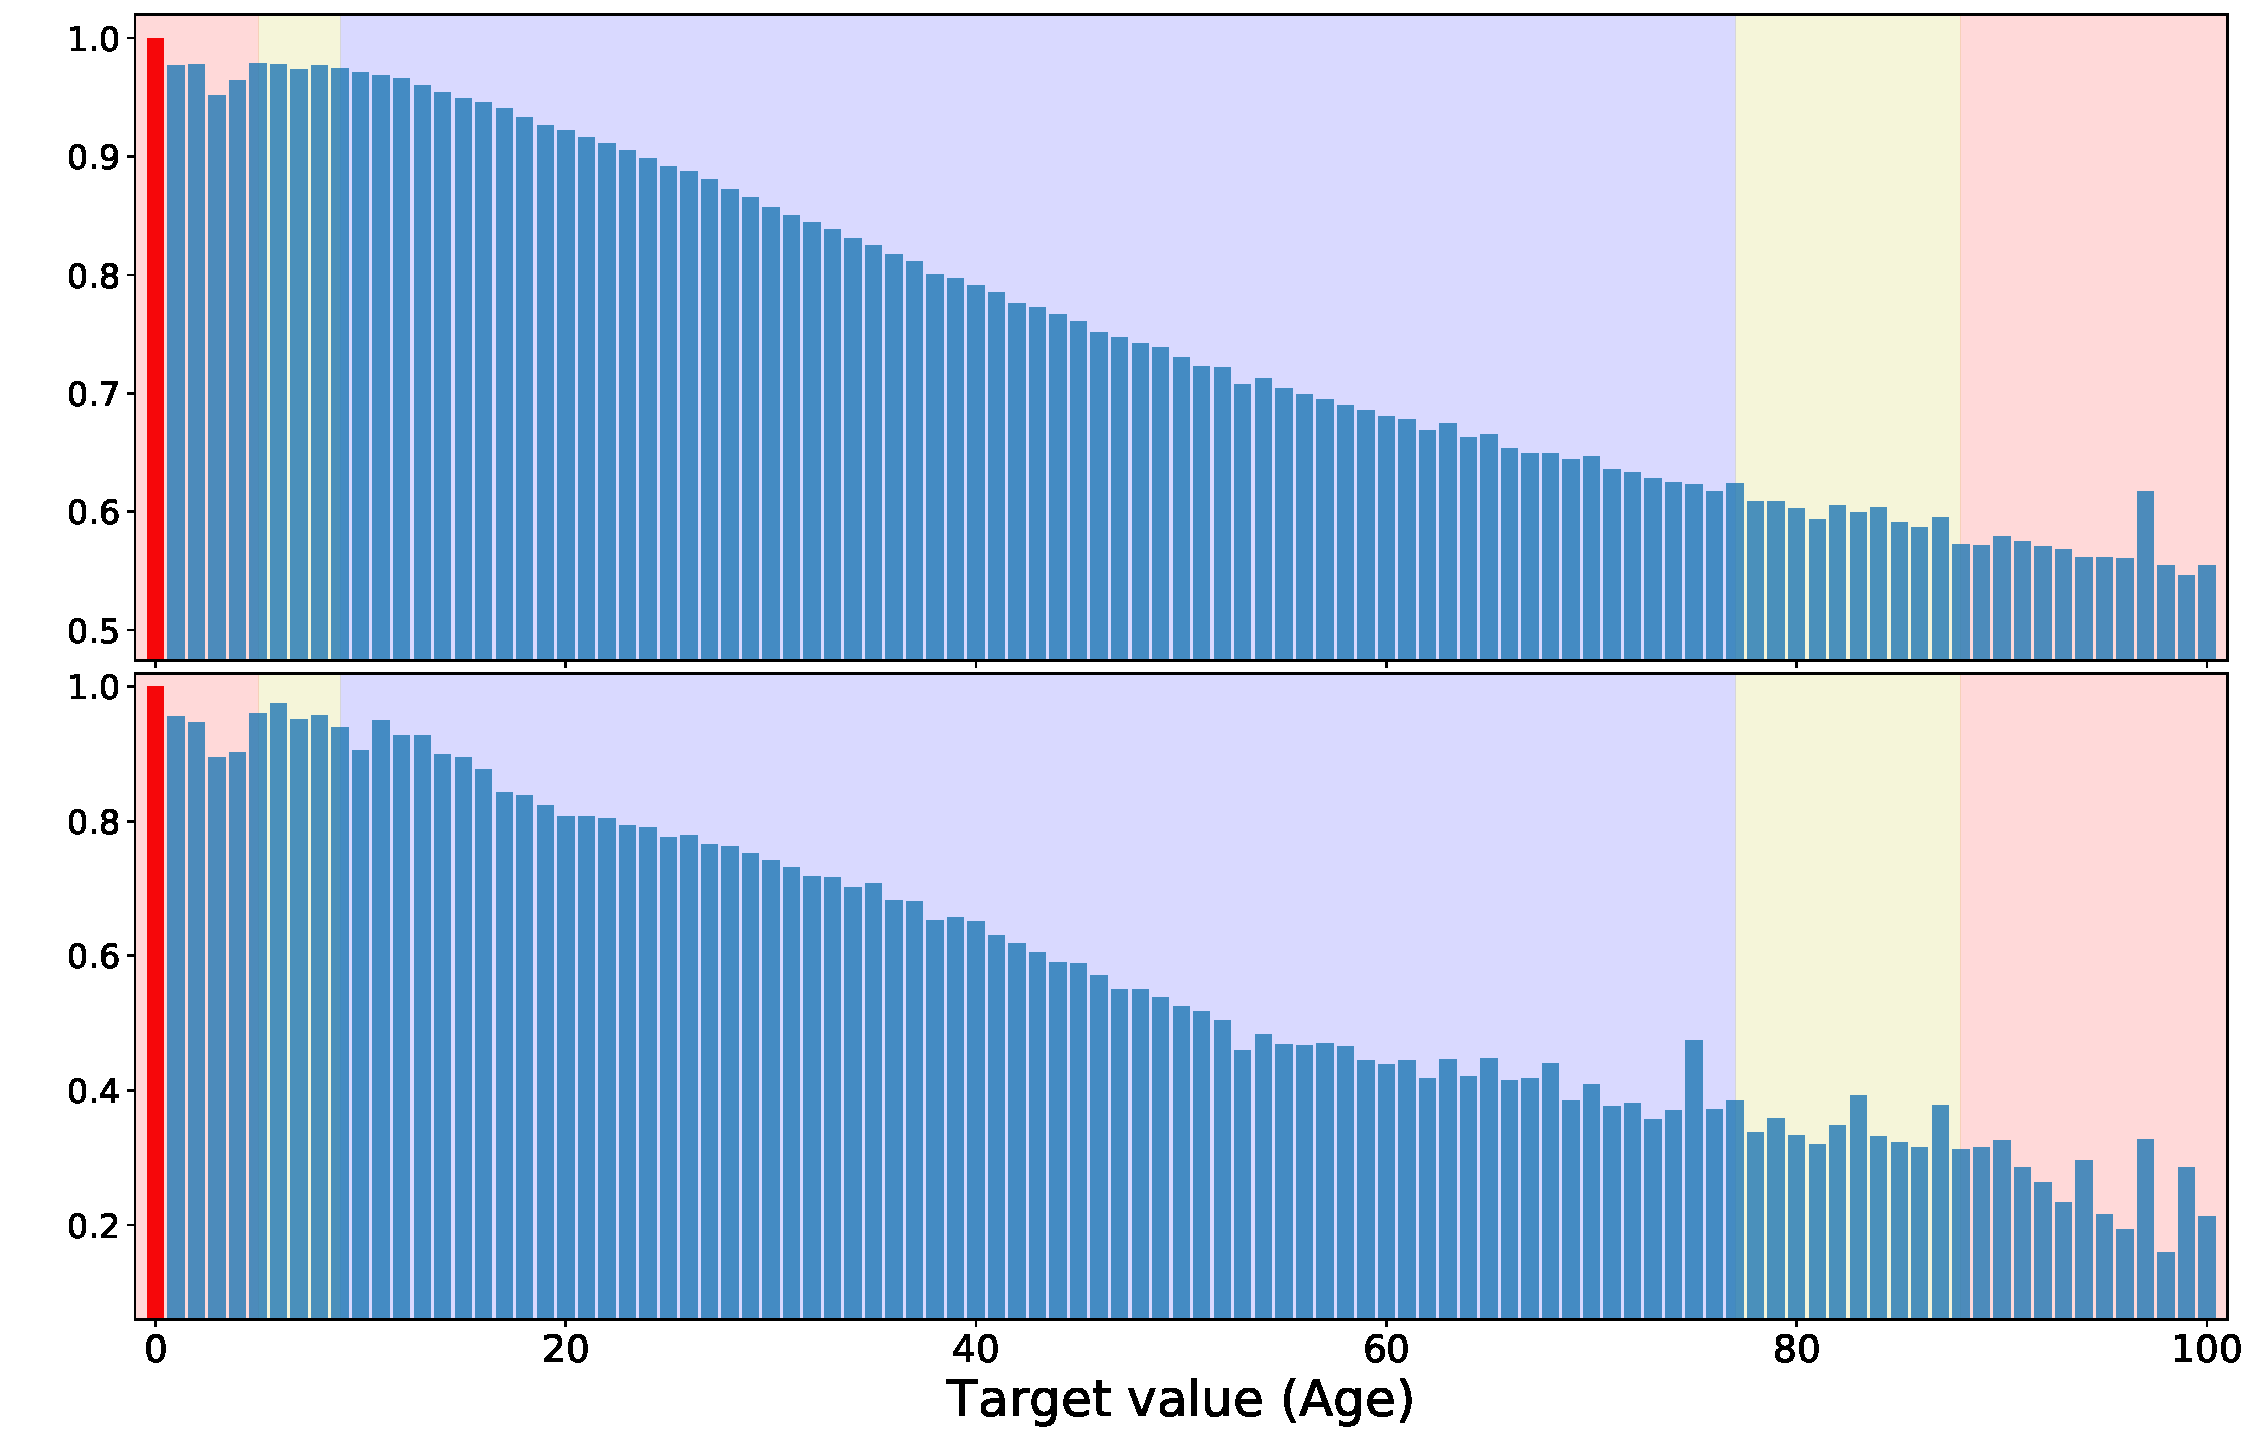
\includegraphics[width=\linewidth]{images/feat_sim_fds_ours_0.pdf}
			\caption{FDS}
		\end{subfigure}
		%\caption{}
	\end{figure}
	\vspace{-1em}
	\begin{columns}
		\footnotesize
		\begin{column}{0.5\textwidth}
			\begin{itemize}
				\item High similarity in neighbourhood for mean
				\item \red{High similarities with further regions}
				\item \red{Lower similarities with some closer regions, e.g., variance neighbourhood}
			\end{itemize}
		\end{column}
		\begin{column}{0.5\textwidth}
			\begin{itemize}
				\item Improved feature statistics calibration:
				\begin{itemize}
					\vspace{-1.5em}
					\scriptsize
					\item High similarity only in neighbourhood
					\item ``The further the region the lower the similarity''
					\item More gradual similarity change
				\end{itemize}
			\end{itemize}
		\end{column}
	\end{columns}
	\credit{Image}{yang2021delving}
\end{frame}

\begin{frame}{Feature statistics similarity (4/4)}{Anchor age 90}
	\begin{figure}[h]
		\begin{subfigure}{0.48\textwidth}
			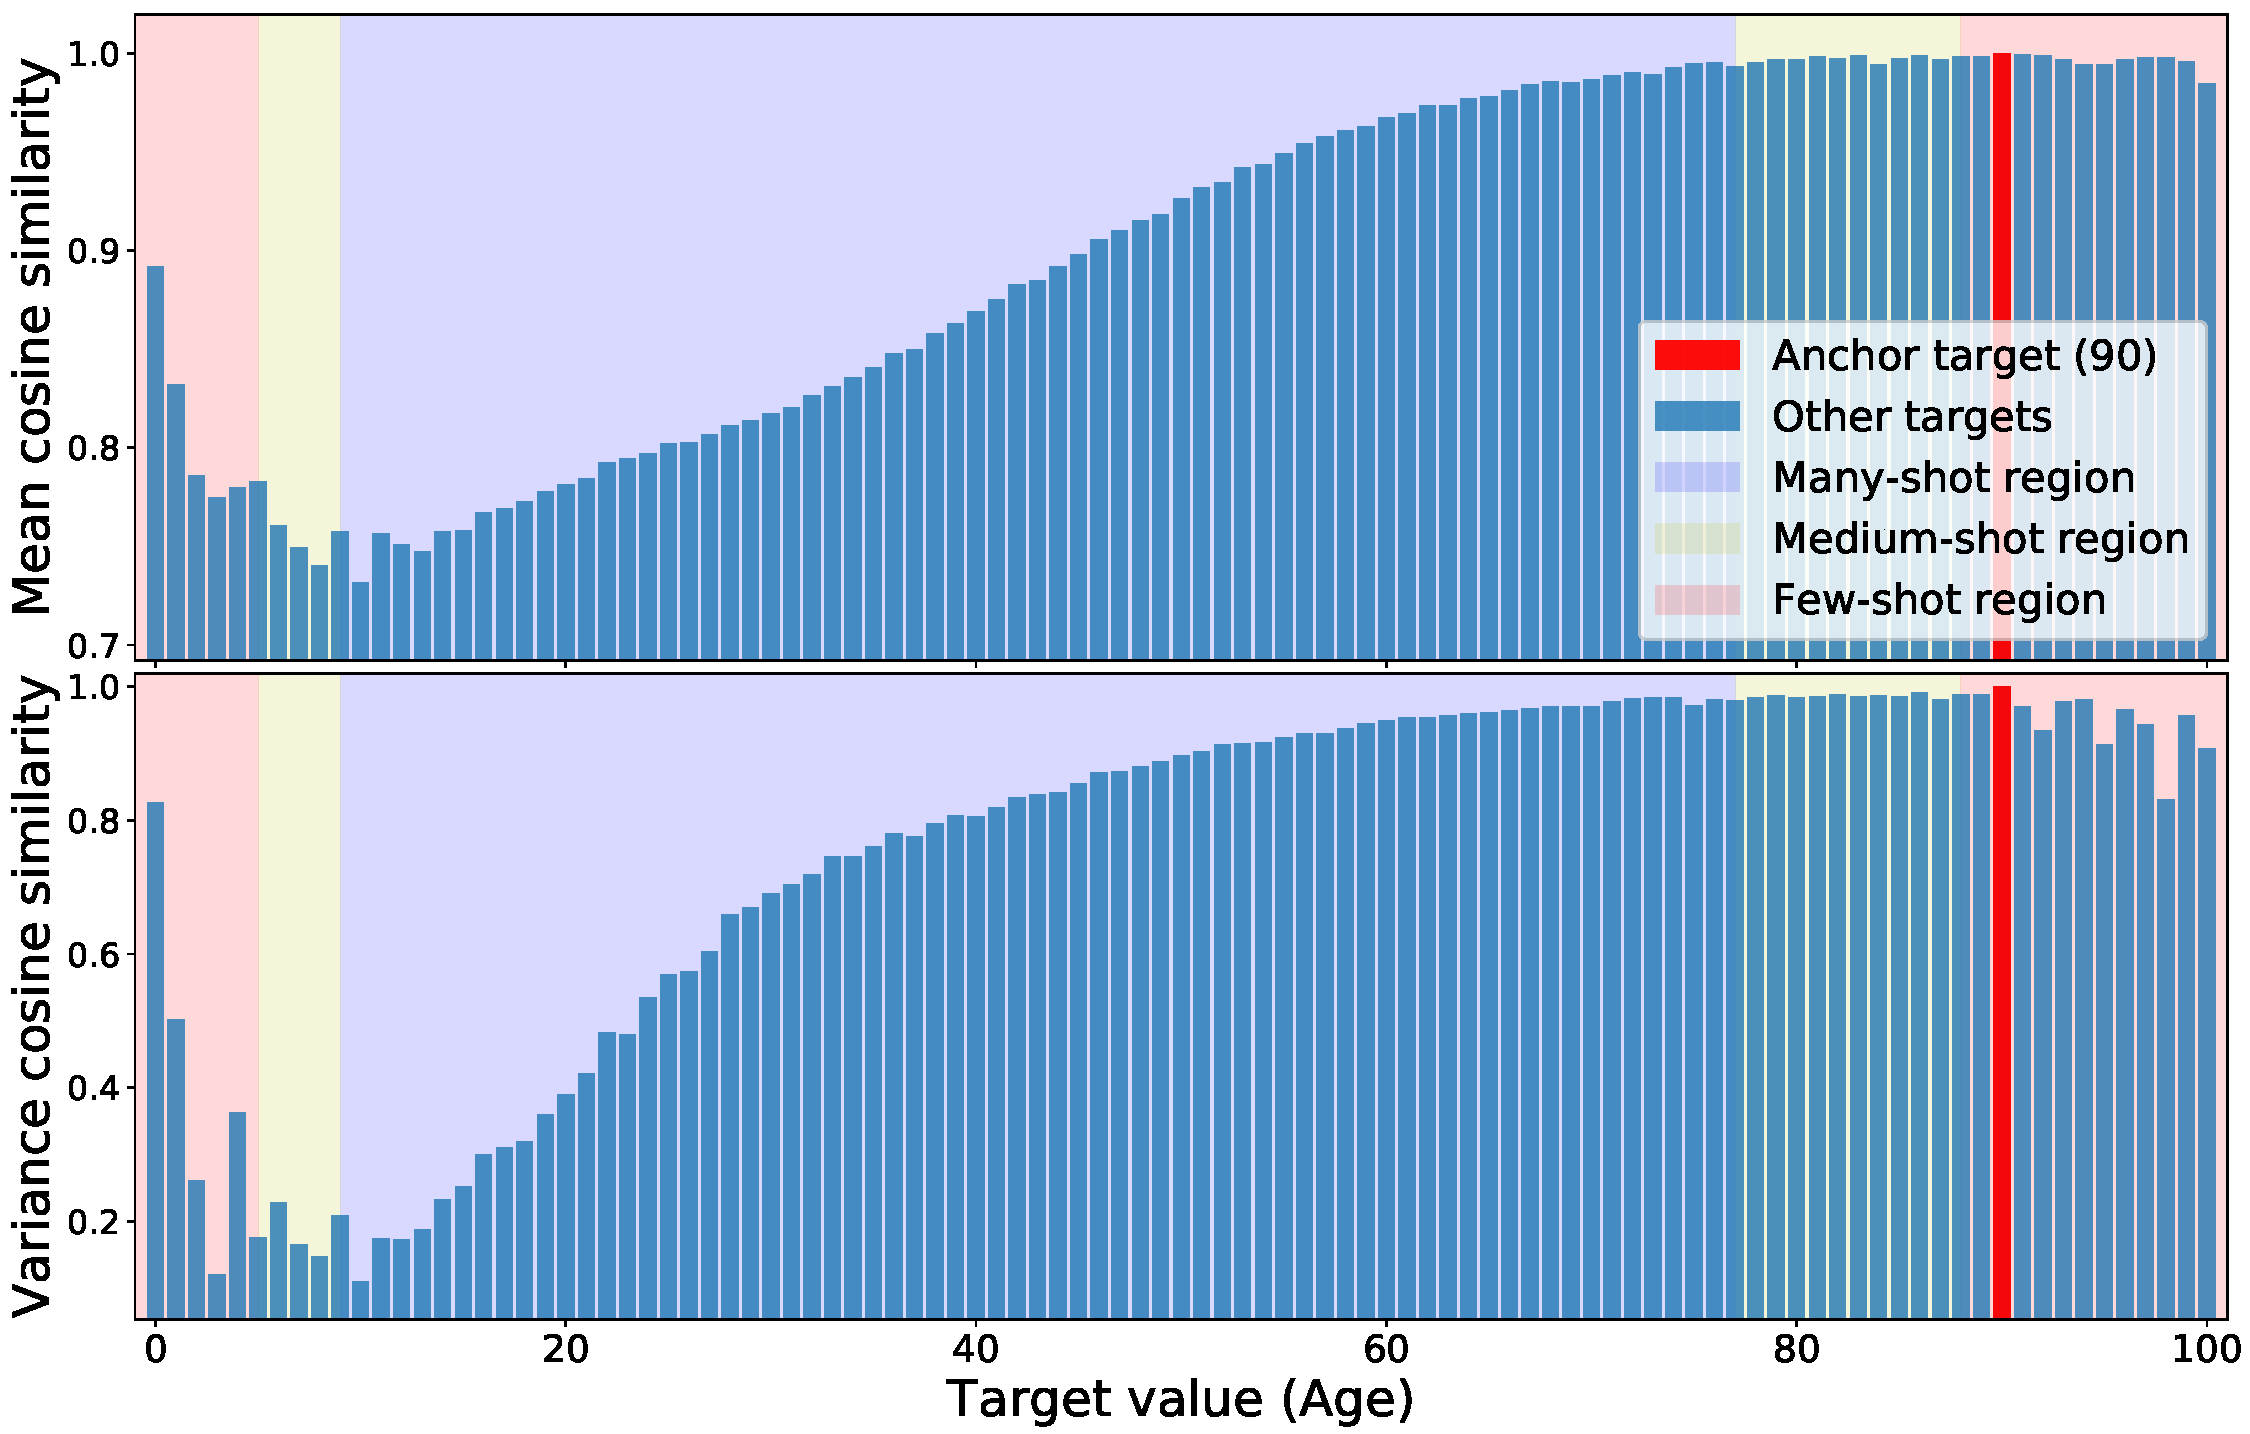
\includegraphics[width=\linewidth]{images/feat_sim_fds_base_90.pdf}
			\caption{Baseline}
		\end{subfigure}\hspace{1em}%
		\begin{subfigure}{0.48\textwidth}
			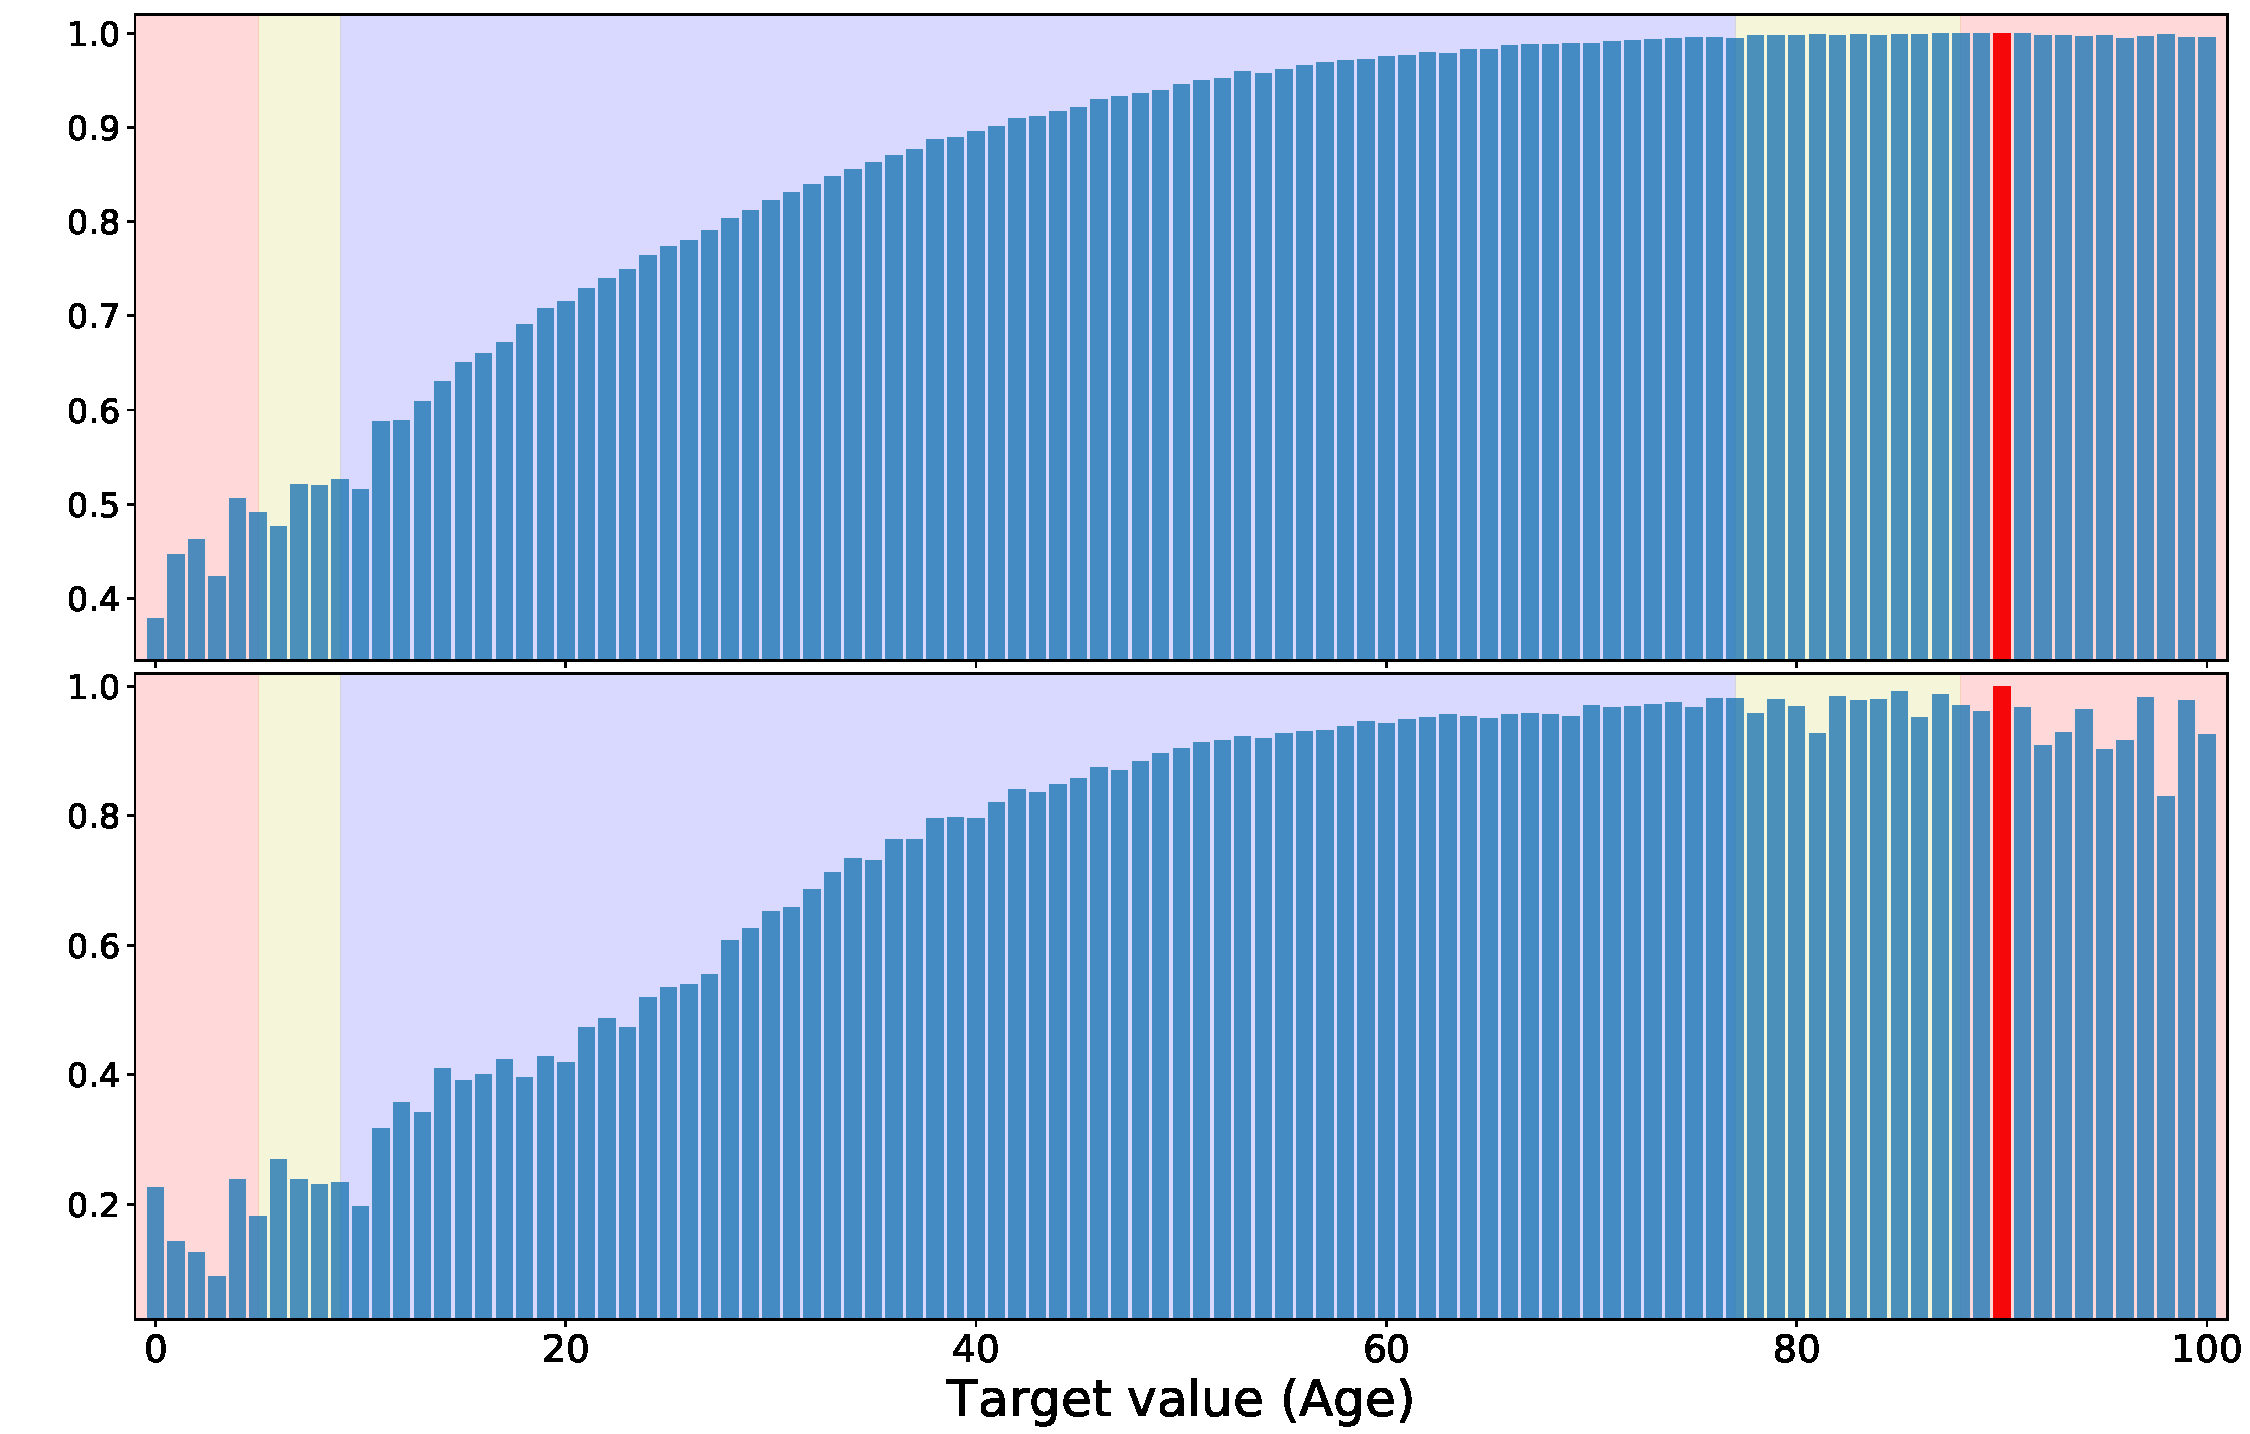
\includegraphics[width=\linewidth]{images/feat_sim_fds_ours_90.pdf}
			\caption{FDS}
		\end{subfigure}
		%\caption{}
	\end{figure}
	\vspace{-1em}
	\begin{columns}
		\footnotesize
		\begin{column}{0.5\textwidth}
			\begin{itemize}
				\item High similarity in neighbourhood, \\esp. for mean
				\item \red{High similarities with further regions}
				\item \red{Lower similarities with some closer regions}
			\end{itemize}
		\end{column}
		\begin{column}{0.5\textwidth}
			\begin{itemize}
				\item Improved feature statistics calibration:
				\begin{itemize}
					\vspace{-1.5em}
					\scriptsize
					\item High similarity only in neighbourhood
					\item ``The further the region the lower the similarity''
					\item More gradual similarity change
				\end{itemize}
			\end{itemize}
		\end{column}
	\end{columns}
	\credit{Image}{yang2021delving}
\end{frame}

\begin{frame}{Change of feature statistics w.r.t. epoch}
	\begin{figure}[h]
		\begin{subfigure}{0.48\textwidth}
			\begin{tikzpicture}
				\node[above=0.95em, right=1.5em] at (current page.west)
				{
					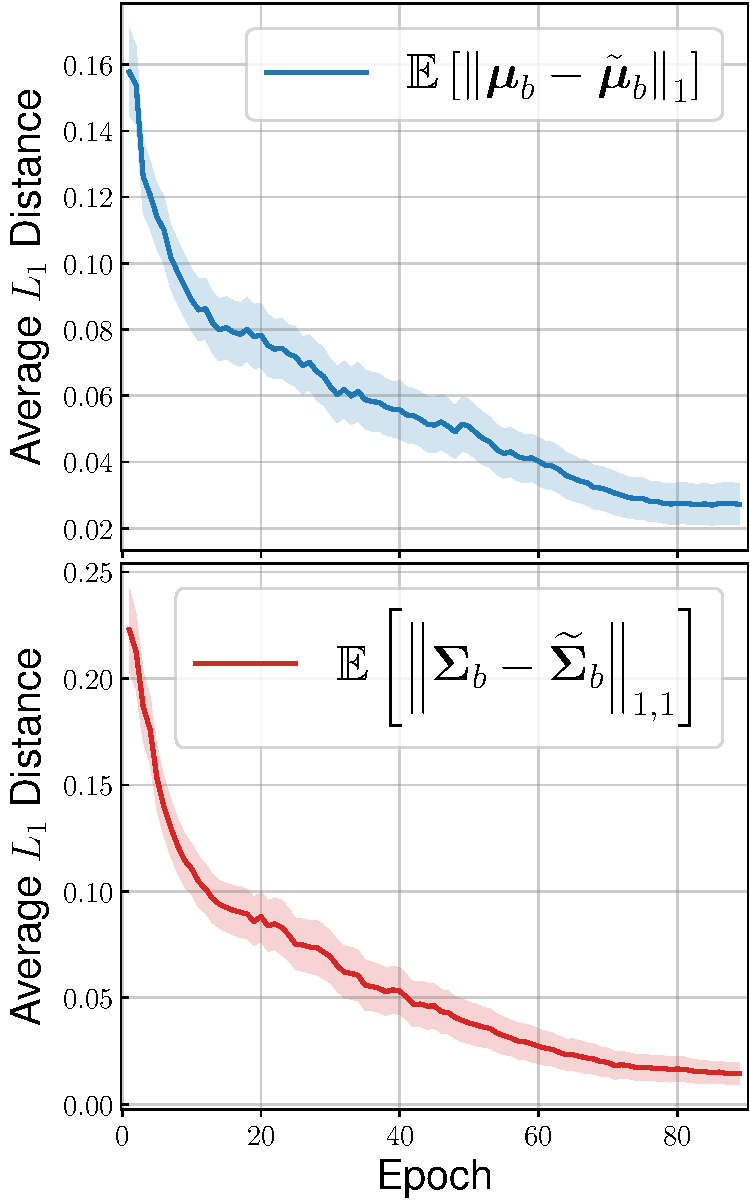
\includegraphics[trim={0 28.5em 0 0},clip,scale=0.4]{images/fds_diff_train.pdf}
				};
				\node[below=4.8em, right=1.5em] at (current page.west)
				{
					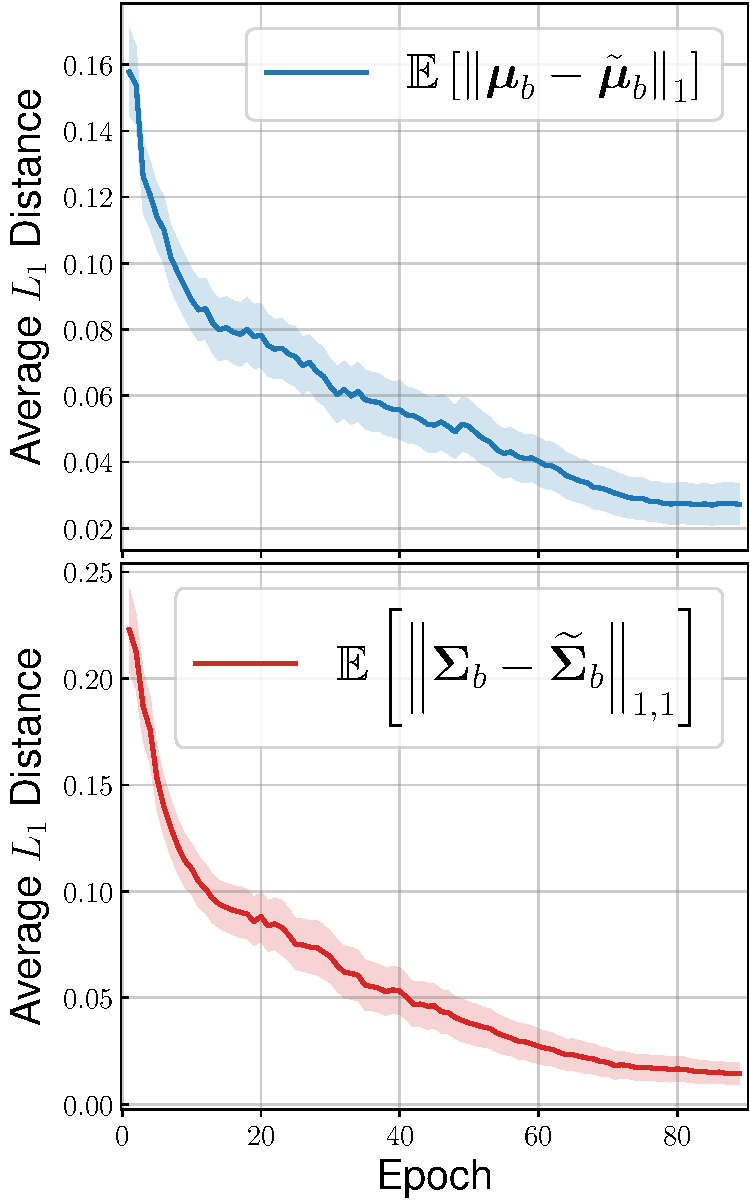
\includegraphics[trim={0 0 0 49.2em},clip,scale=0.4]{images/fds_diff_train.pdf}
				};
			\end{tikzpicture}
			\caption{Mean}
		\end{subfigure}\hspace{1em}%
		\begin{subfigure}{0.48\textwidth}
			\begin{tikzpicture}
				\node[left=1.5em] at (current page.east) 
				{
					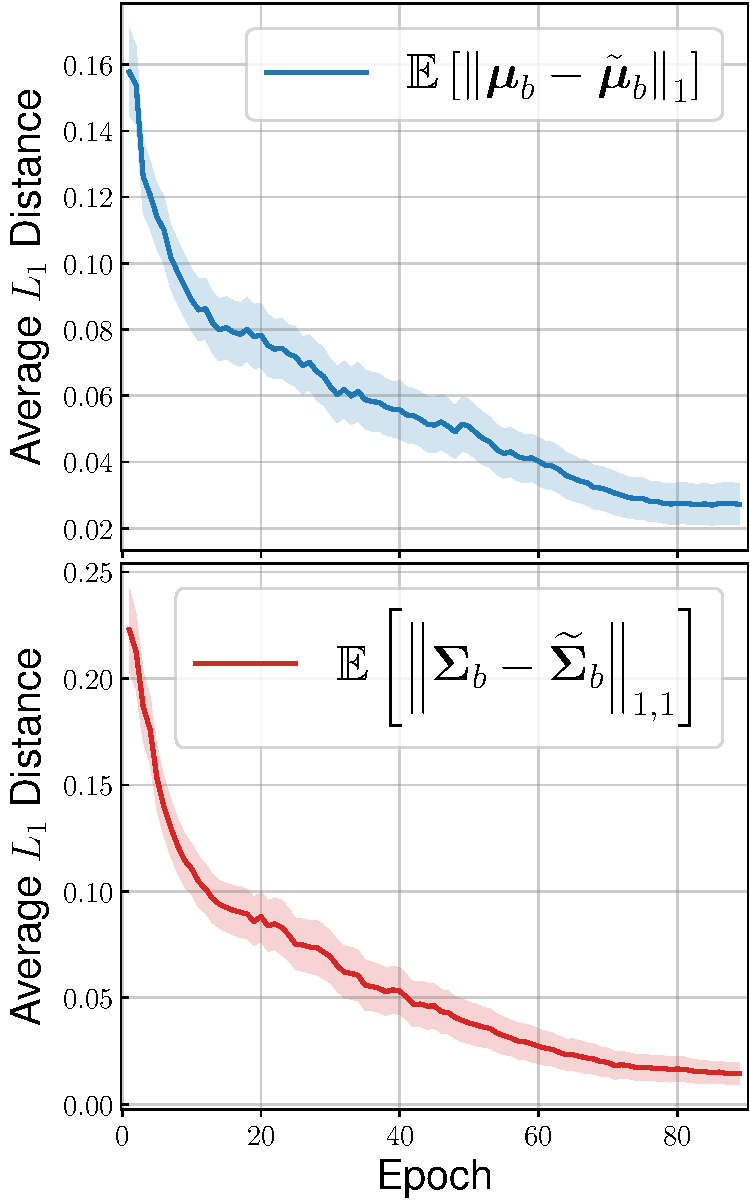
\includegraphics[trim={0 0 0 24.7em},clip,scale=0.4]{images/fds_diff_train.pdf}
				};
			\end{tikzpicture}
			\caption{Variance}
		\end{subfigure}
		%\caption{}
	\end{figure}
	\begin{itemize}
		\item ${\bm{\mu}, \bm{\Sigma}}$: Running mean and variance
		\item ${\bm{\tilde{\mu}}, \bm{\tilde{\Sigma}}}$: Smoothed mean and variance
	\end{itemize}
	\credit{Image}{yang2021delving}
\end{frame}

\begin{frame}{The FDS Algorithm}
	\begin{figure}[h]
		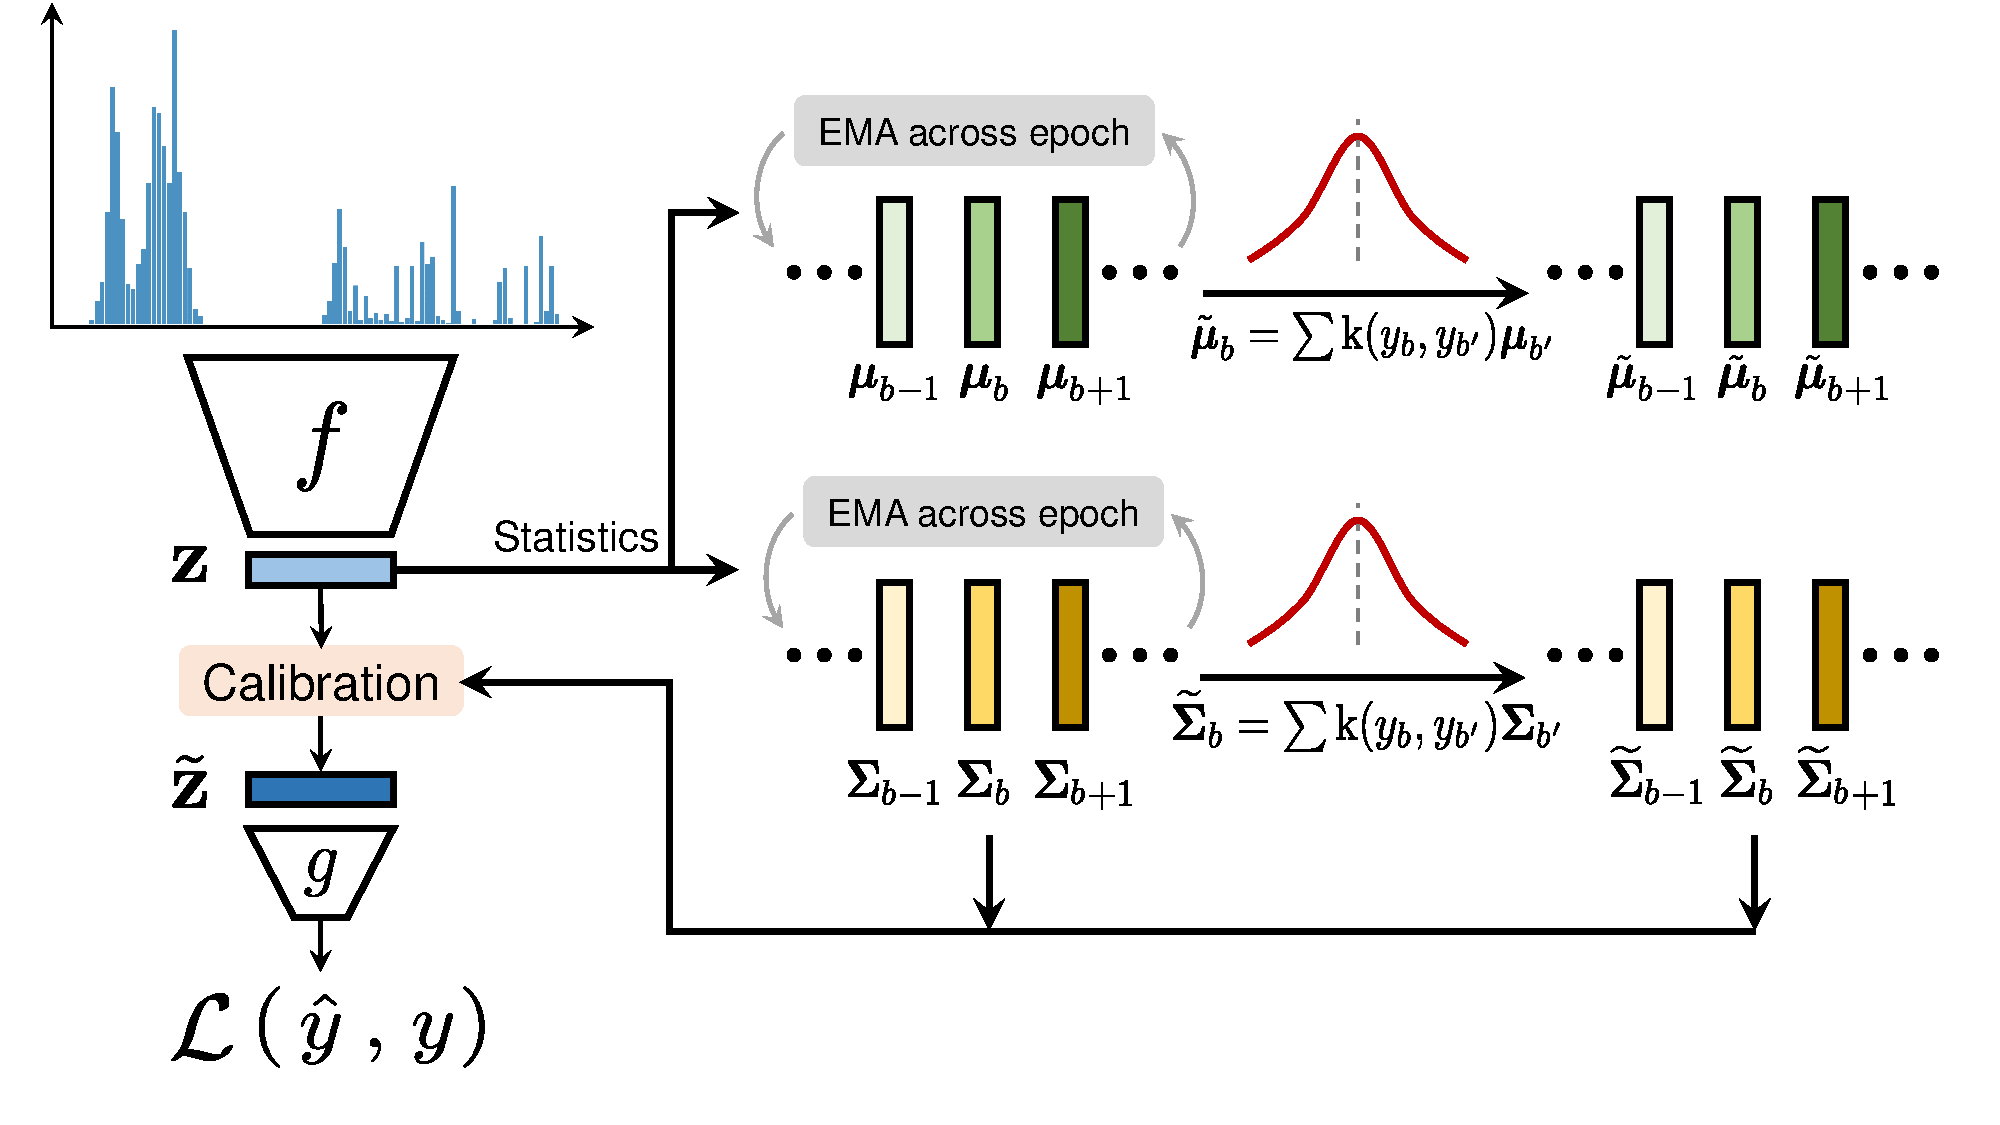
\includegraphics[width=\linewidth]{images/teaser_fds.pdf}
		%\caption{}
	\end{figure}
	\credit{Image}{yang2021delving}
\end{frame}